\documentclass{article}
% ----- Preamble
\usepackage[utf8]{inputenc} % police encodee en latin1=iso8859-1=Windows Latin 1 %
\usepackage[french]{babel} % police fr %
\usepackage{hyperref} % pour les references %
\usepackage{amsmath} % pour les formules de maths %
\usepackage{amssymb} % pour les symboles maths %
\usepackage{amsthm} % pour la mise en forme des theoremes %
\usepackage{aeguill} % pour les guillemets et accents francais %
\usepackage{listings} % pour les listings de code %
\usepackage{helvet} % police helvetica %
\usepackage{graphicx}
\usepackage{dsfont}
\usepackage{subcaption}
\usepackage{caption}
% modification des dimensions de la page et de son centrage %
\topmargin 0.0cm
\oddsidemargin 0.1cm
\textwidth 16cm 
\textheight 22cm
\footskip 0.0cm

\title{Traitement d'Image et du Signal - TP6}
\author{Laurent Cetinsoy, Karim Kouki, Aris Tritas }
\date{\today}

\begin{document}
\maketitle

\section{Echange de phase}

Dans cette partie on s'intéresse à l'information portée par la phase et le module de la TFD d'une image. 


\begin{figure}[h]
	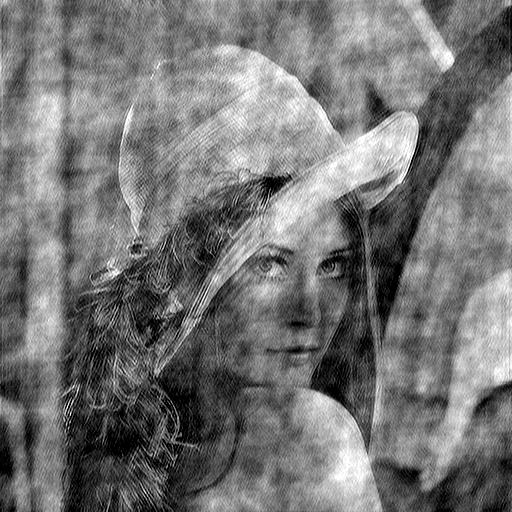
\includegraphics[width=0.3\textwidth]{phase_swapping.jpg}
	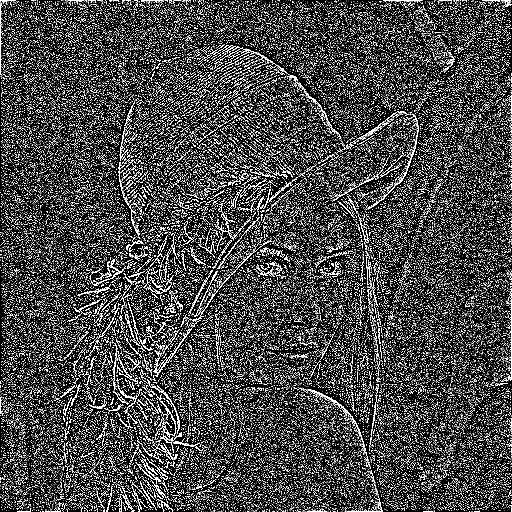
\includegraphics[width=0.3\textwidth]{phase_swapping_in_random.jpg}
	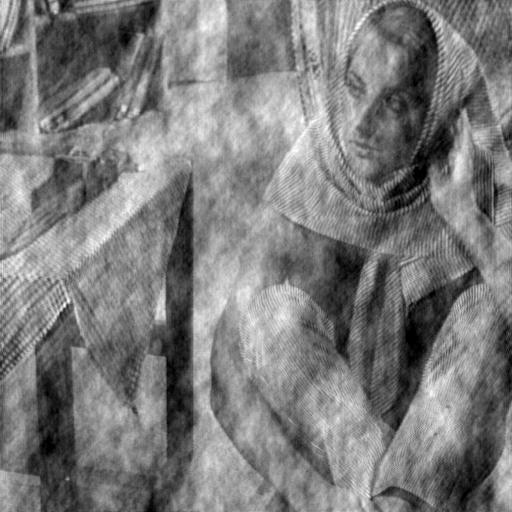
\includegraphics[width=0.3\textwidth]{module_swapping.jpg}

  \caption{A gauche la phase de lena qui a été mélangée au module de barbara. Au milieu, la phase de lena projetée sur une image générée par une gaussienne. A droite le module de Lena et Barbara ont été échangés.}
\end{figure}

On constate qu'une grande partie de l'information est portée par la phase. Inversement on voit que si on transfère le module de l'image de Lena dans Barbara, on voit bien barbara (qui est quand même moins sexy). 

Néanmoins la phase seule ne suffit pas (cf figure.2) : si on transporte la phase sur une image uniforme, l'image reste inchangée après transport de phase. 

\begin{figure}[h]

	
\includegraphics[width=0.3\textwidth]{phase_swapping_in_grey_image.jpg}

  \caption{Phase de lena exportée dans une image constante (gris total)}
\end{figure}


On voit que le module ne porte que peu d'information mais a quand même besoin d'être présent. 


\section{Ré-haussement des couleurs}

\section{Changement de contraste}

\subsection*{Question 1}

\begin{figure}[h]

	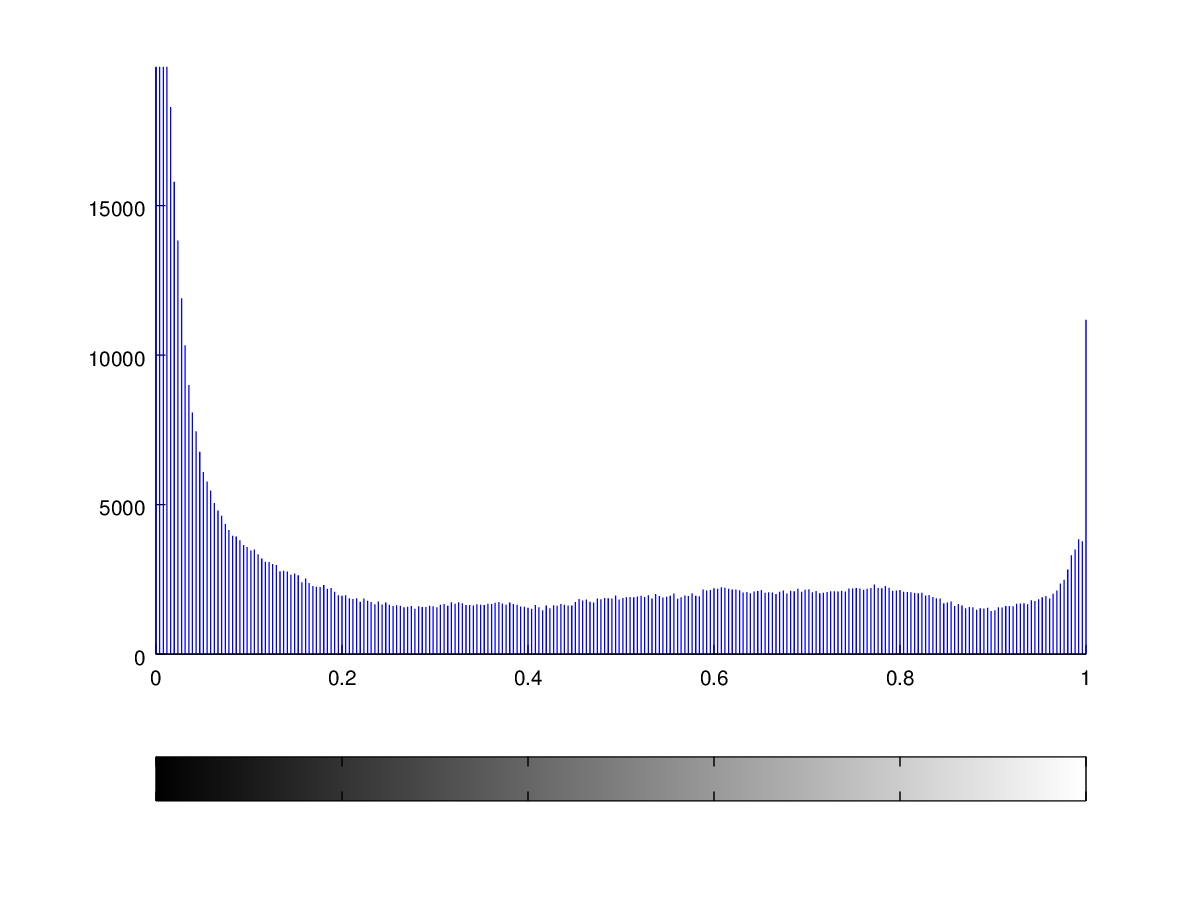
\includegraphics[width=0.5\textwidth]{hist_orig.png}
	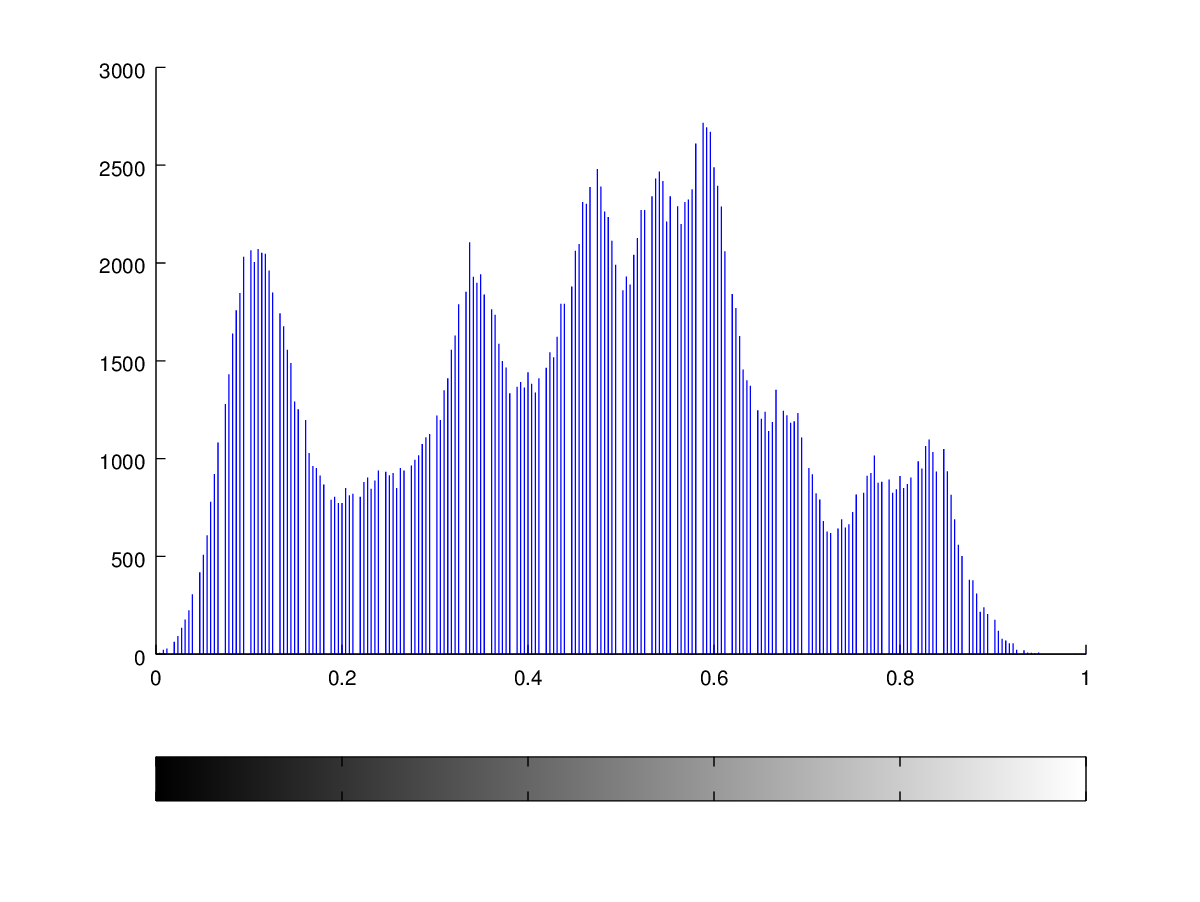
\includegraphics[width=0.5\textwidth]{hist_scaled.png}
		
	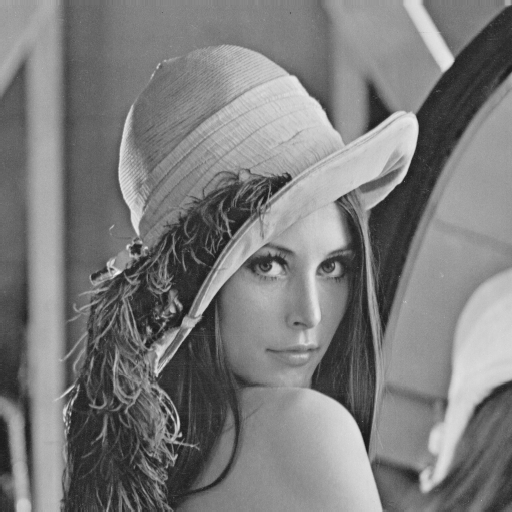
\includegraphics[width=0.5\textwidth]{lena.png}
	\includegraphics[width=0.5\textwidth]{lena_hist_scaled.png}
		
	\caption{A gauche l'image et l'histogramme originaux. A droite après changement de contraste affine}
	
\end{figure}

\subsection*{Question 2}

Dans le cas où il existe dans l'image un pixel qui est nul et un pixel d'intensité maximal (1). Alors la transformation affine n'a aucun effet : 


$$min(I(i,j) = 0$$
$$max(I(i,j)) = 1$$
	
$$I'(i,j) = \frac{1}{min-max} * (I(i,j) - min) = I(i,j)$$


\begin{figure}[h]
		
	\caption{A gauche l'image et l'histogramme originaux. A droite après changement de contraste affine}
	
\end{figure}


On peut remplacer $min(I(i,j)$ par $min(I(i,j)) + \epsilon$ et $max$ par $max(I(i,j)$ par $max(I(i,j) - \epsilon$ (à Tester)


\section{Filtre médian}

\section{Exercice}
\subsection{TF}
$$ f_K : \mathbb{R} \ni x \rightarrow \frac{\mathds{1}_{[0, K]}(x)}{K}, K \in \mathbb{R}_*^+ $$
$$ \hat{f}(\xi) = \int_\mathbb{R} f(x) e^{-ix\xi}$$
\subsection{Convolution}
\end{document}